%!TEX root = ../rapport.tex

\section{Conception}
\label{section:conception_serveur}

Cette section décrit la conception qui a été faite pour aider au mieux durant la phase d'implémentation.


\subsection{Architecture du système}
La figure \ref{gra:archiServeur} illustre l'architecture du serveur qui est composée de deux parties bien distinctes : 

\medskip

\begin{itemize}
	\item Le \emph{\gls{webservice}} de type \emph{\gls{rest}}
	\item La base de données \emph{\gls{mysql}}
\end{itemize}


\begin{figure}[H]
      \centering
      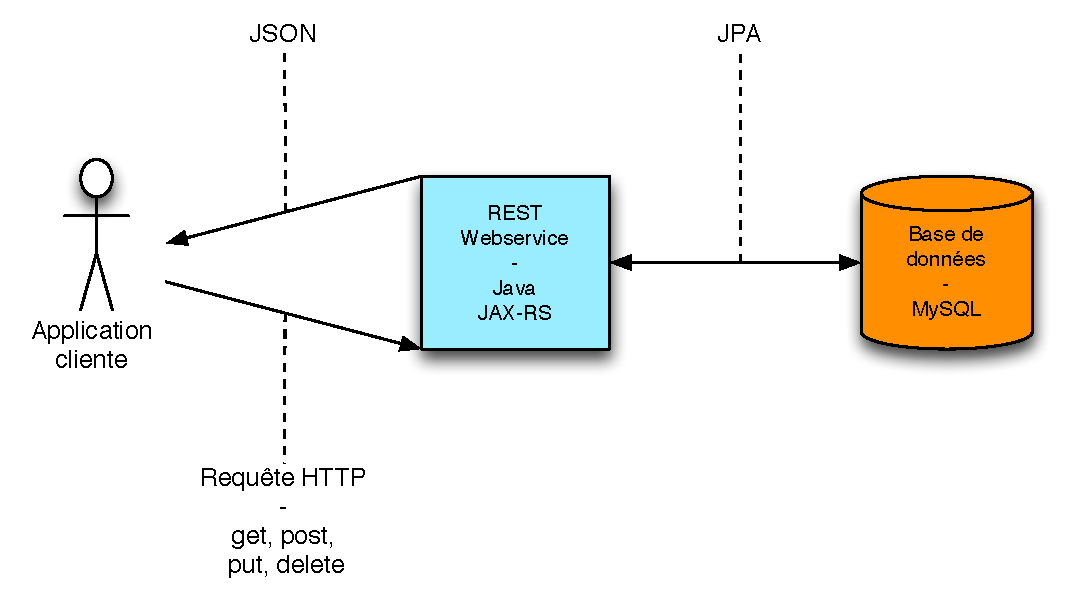
\includegraphics[width=14cm]{00_media/04_Serveur_archi.pdf}
      \caption{Architecture du serveur}
      \label{gra:archiServeur}
\end{figure}

L'application cliente requête le \emph{\gls{webservice}} à l'aire du protocole \emph{\gls{http}} et peut employer des types de méthodes comme \emph{get, post, put, delete}.

\medskip

L'application cliente reçoit les réponses au format \emph{\gls{json}} et se charge des les transformer selon ses besoins.

\medskip

Le \emph{\gls{webservice}} est de type \emph{\gls{rest}} et est implémenté avec \emph{\gls{jaxrs}} qui est une interface de programmation \emph{\gls{java}} permettant de créer des \emph{\glspl{webservice}}.

\medskip

Le tout s'articule autour d'une base de données \emph{\gls{mysql}} qui permet d'enregistrer les données en utilisant \emph{\gls{jpa}}.

\subsection{Architecture du webservice} % (fold)
\label{sub:architecture_du_webservice}
Pour expliquer l'architecture et la structure du \emph{\gls{webservice}}, je vais m'aider de la figure \ref{gra:gethouselistsequence} qui est un diagramme de séquence très simple destiné à pouvoir, au fil du voyage de la requête, détaillé le processus. 

\begin{figure}[H]
      \centering
      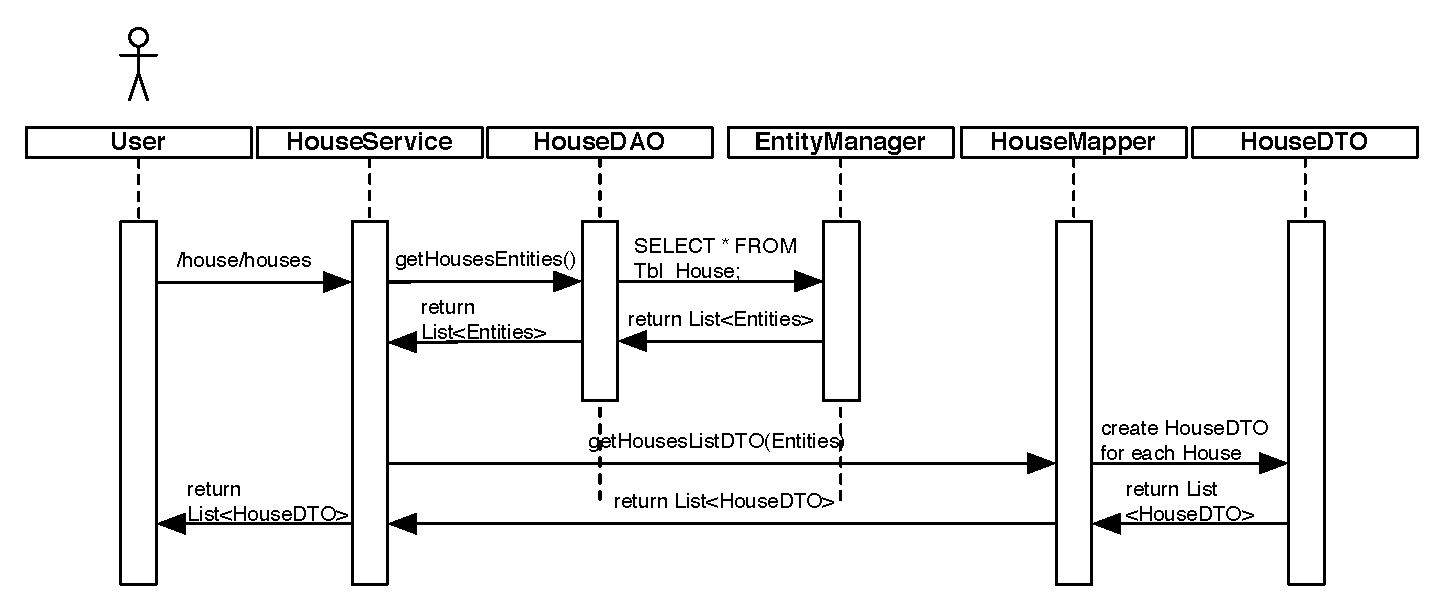
\includegraphics[width=\textwidth]{00_media/04_SequenceGetHousesList.pdf}
      \caption{Diargramme de séquence - GET Houses List}
      \label{gra:gethouselistsequence}
\end{figure}

L'utilisateur fait donc une requête sur le webservice à l'aide d'une fin d'\emph{\gls{url}} du type \emph{/house/houses}. La classe \texttt{HouseService} implémentée en \emph{\gls{jersey}} interroge la classe \texttt{HouseDAO} en lui demande de lui retourner toutes les entités. Elle attend donc une liste d'entités en retour. La classe \texttt{HouseDAO} se charge de sélectionner les entrées dans la base de données et les retournes sous formes de liste. Une fois la réponse arrivée à la classe \texttt{HouseService}, elle se charge de demander à la classe \texttt{HouseMapper} une liste qu'elle puisse retourner à l'utilisateur avec le bon format. La classe \texttt{HouseMapper} travaille avec \texttt{HouseDTO} qui permettra justement de faire ceci. Finalement, l'utilisateur reçoit sa réponse.

% subsection architecture_du_webservice (end)

\subsection{REST API pour l'application} % (fold)
\label{sub:rest_api_pour_l_application}
Cette section décrit l'interface (\emph{\gls{api}}) que doit fournir le \emph{\gls{webservice}} pour que toutes les opérations de l'application cliente soient possibles.

\medskip

L'\emph{\gls{api}} a été séparée en différentes parties afin de mieux cibler chacune d'elle, à savoir : 

\medskip

\begin{itemize}
	\item Login
	\item Maisons
	\item Zones
	\item Capteurs
	\item Données des capteurs
\end{itemize}

\medskip

Afin de rendre les tableaux qui suivent plus légers, toutes les \gls{url} doivent être précédées par \url{http://adresse:port/ga-service} pour fonctionner.

\subsubsection{Login}
Le tableau \ref{tab:apiLogin} permet de savoir comment utiliser le \emph{\gls{webservice}} pour recevoir et envoyer les informations de login.

\begin{table}[H]
\begin{tabularx}{\textwidth}{|X|X|X|X|X|}
  \hline
  \bf{Nom}  & \bf{URL} & \bf{Type} & \bf{Paramètres} & \bf{Retour} \\
  \hline  
  Se loguer  & /token/ask & GET &  user, password & Pas OK -> error 404 OK --> User \emph{\gls{json}}\\
  \hline  
  Contrôle login & /token/check & GET & token  & true, false\\
  \hline  
  Se délogguer & /token/logout & GET & token  & true, false\\
  \hline  
\end{tabularx}
\caption{API du webservice - Login}
\label{tab:apiLogin}
\end{table}

\subsubsection{Maisons}
Le tableau \ref{tab:apiMaison} permet de savoir comment utiliser le \emph{\gls{webservice}} pour recevoir et envoyer les informations sur les maisons.

\begin{table}[H]
\begin{tabularx}{\textwidth}{|X|m{3cm}|X|X|X|}
  \hline
  \bf{Nom}  & \bf{URL} & \bf{Type} & \bf{Paramètres} & \bf{Retour} \\
  \hline  
  Toutes les maisons  & /house/houses & GET &  - & Liste des maisons \emph{\gls{json}} \\
  \hline
 Les maisons d'un utilisateur  & /house/user/\{id\} & GET &  id & Liste des maisons \emph{\gls{json}} \\
  \hline 
 Créer une maison  & /house/create & POST & House \emph{\gls{json}} & House \emph{\gls{json}} \\
  \hline 
 Modifier une maison  & /house/update & POST & House \emph{\gls{json}} & House \emph{\gls{json}} \\
  \hline   
 Supprimer une maison  & /house/delete/\{id\} & DELETE &  id & error 404 ou 200 \\
  \hline  
\end{tabularx}
\caption{API du webservice - Maison}
\label{tab:apiMaison}
\end{table}

\subsubsection{Zones}
Le tableau \ref{tab:apiZone} permet de savoir comment utiliser le \emph{\gls{webservice}} pour recevoir et envoyer les informations sur les zones.

\begin{table}[H]
\begin{tabularx}{\textwidth}{|X|X|X|X|X|}
  \hline
  \bf{Nom}  & \bf{URL} & \bf{Type} & \bf{Paramètres} & \bf{Retour} \\
  \hline  
  Toutes les zones  & /zone/zones & GET &  - & Liste des zones \emph{\gls{json}} \\
  \hline
 Les zones d'une maison  & /zone/house/\{id\} & GET &  id & Liste des maisons \\
  \hline 
 Créer une zone  & /zone/save & POST & Zone \emph{\gls{json}} & Zone \emph{\gls{json}} \\
  \hline 
 Modifier une zone  & /zone/updateZone & POST & Zone \emph{\gls{json}} & Zone \emph{\gls{json}} \\
  \hline   
 Supprimer une zone  & /zone/delete/\{id\} & DELETE &  id & error 404 ou 200 \\
  \hline  
\end{tabularx}
\caption{API du webservice - Zone}
\label{tab:apiZone}
\end{table}

\subsubsection{Capteurs}
Le tableau \ref{tab:apiCapteur} permet de savoir comment utiliser le \emph{\gls{webservice}} pour recevoir et envoyer les informations sur les capteurs.

\begin{table}[H]
\begin{tabularx}{\textwidth}{|X|m{3cm}|X|X|X|}
  \hline
  \bf{Nom}  & \bf{URL} & \bf{Type} & \bf{Paramètres} & \bf{Retour} \\
  \hline  
  Tous les capteurs  & /sensor/sensors & GET &  - & Liste des capteurs \emph{\gls{json}} \\
  \hline
 Les capteurs d'une zone  & /sensor/zone/\{id\} & GET &  id & Liste des capteurs \\
  \hline 
 Modifier un capteur  & /sensor/update & PUT & Sensor \emph{\gls{json}} & Sensor \emph{\gls{json}} \\
  \hline   
   Retirer d'une zone & /sensor/noZone & POST &  Sensor \emph{\gls{json}} & Sensor \\
  \hline  
\end{tabularx}
\caption{API du webservice - Capteur}
\label{tab:apiCapteur}
\end{table}

\subsubsection{Données des capteurs}
Le tableau \ref{tab:apiCapteurData} permet de savoir comment utiliser le \emph{\gls{webservice}} pour recevoir les données des capteurs.

\begin{table}[H]
\begin{tabularx}{\textwidth}{|X|X|X|X|X|}
  \hline
  \bf{Nom}  & \bf{URL} & \bf{Type} & \bf{Paramètres} & \bf{Retour} \\
  \hline  
  Les données pour un capteur  & /sensorData/sensor/{id} & GET &  id & Liste des données \emph{\gls{json}} \\
  \hline
 Les dernières données pour un capteur  & /sensorData/sensor/\{id\}/last & GET & id & Liste des données \emph{\gls{json}} \\
  \hline 
\end{tabularx}
\caption{API du webservice - Données du capteur}
\label{tab:apiCapteurData}
\end{table}
% subsection rest_api_pour_l_application (end)